\chapter{Weighting Scheme 1 Supplementaries}
\label{chap:apdx_weights}
Below, we summarize some investigations that exclude various possible explanations for the observed deviations in $w_2(\eta)$ (Scheme 1) that we established in Chap.~\ref{chap:weights}.

\section{Influence of Polarizations}
Theoretically, polarizations could cause deviations, when not properly reproduced in simulated events.
The significant polarization of the \Lz particle in \decay{\Lb}{\jpsi\Lz} was predicted~\cite{LbToJpsiLz_thpol} and measured by the \lhcb collaboration~\cite{LbToJpsiLz_polarization}.
However, assuming \CP conservation, polarization effects should cancel exactly for \Lb and \Lbbar.
Since the weighting procedure outlined above considers combined data sets of \Lb and \Lbbar (raw asymmetry in data $1 - n(\Lb)/n(\Lbbar) = -3.9(1.9)\,\%$ for \gls{LL} and $-8.4(1.6)\,\%$ for \gls{DD}) and no enhancement is observed in $\eta(\Lb)$ distributions where samples where explicitly split w.r.t.\ the proton charge, we exclude that polarization effects introduce such an effect.

\section{Influence of Misalignment}
A major difference to the final state particles \proton\pim in \decay{\Lb}{\Dz\proton\pim} is that the origin vertex of \proton\pim in \decay{\Lb}{\jpsi\Lz} is well displaced, even for \gls{LL} tracks.
Large values of the $z$-position of the \Lz decay vertex correspond to the case that less layers of the \gls{velo} are passed by the final state particles and the sensitivity to misalignment effects become stronger.
We therefore consider the double ratio of recorded data and \gls{mc} simulated events for $\eta < 3.25$ and $\eta \ge 3.25$:
\begin{multline*}
    \frac{\mathrm{d}}{\mathrm{d}z} \left( \frac{\mathrm{data}, \, \eta(\Lambda_b) < 3.25}{\mathrm{MC}, \, \eta(\Lambda_b) < 3.25} \middle/ \frac{\mathrm{data}, \, \eta(\Lambda_b) \ge 3.25}{\mathrm{MC}, \, \eta(\Lambda_b) \ge 3.25} \right) < 0 \\
    \Leftrightarrow \quad \text{missing MC events for $\eta > 3.25$ and large $z$}.
\end{multline*}
The normalized double ratio and a fit of a linear function $f(x|c_1,c_2) = c_1 + c_2 x$ is shown in Fig.~\ref{fig:LbToJpsiLz_hdratio_Lz_endvtx}.
The uncertainty band of the fit is calculated by ordinary error propagation
\begin{equation*}
    u_f = \sqrt{\sum_{ij} \left( \frac{\partial f}{\partial c_i} \frac{\partial f}{\partial c_j} \right)^2 \operatorname{cov}(c_i, c_j)} = \sqrt{u_{c_1}^2 + x^2 u_{c_2}^2 + 2x \, \operatorname{cov}(c_1, c_2)} \,.
\end{equation*}
No tension for a preferred slope is visible w.r.t.\ the given uncertainties.

\begin{figure}[htbp]
    \centering
    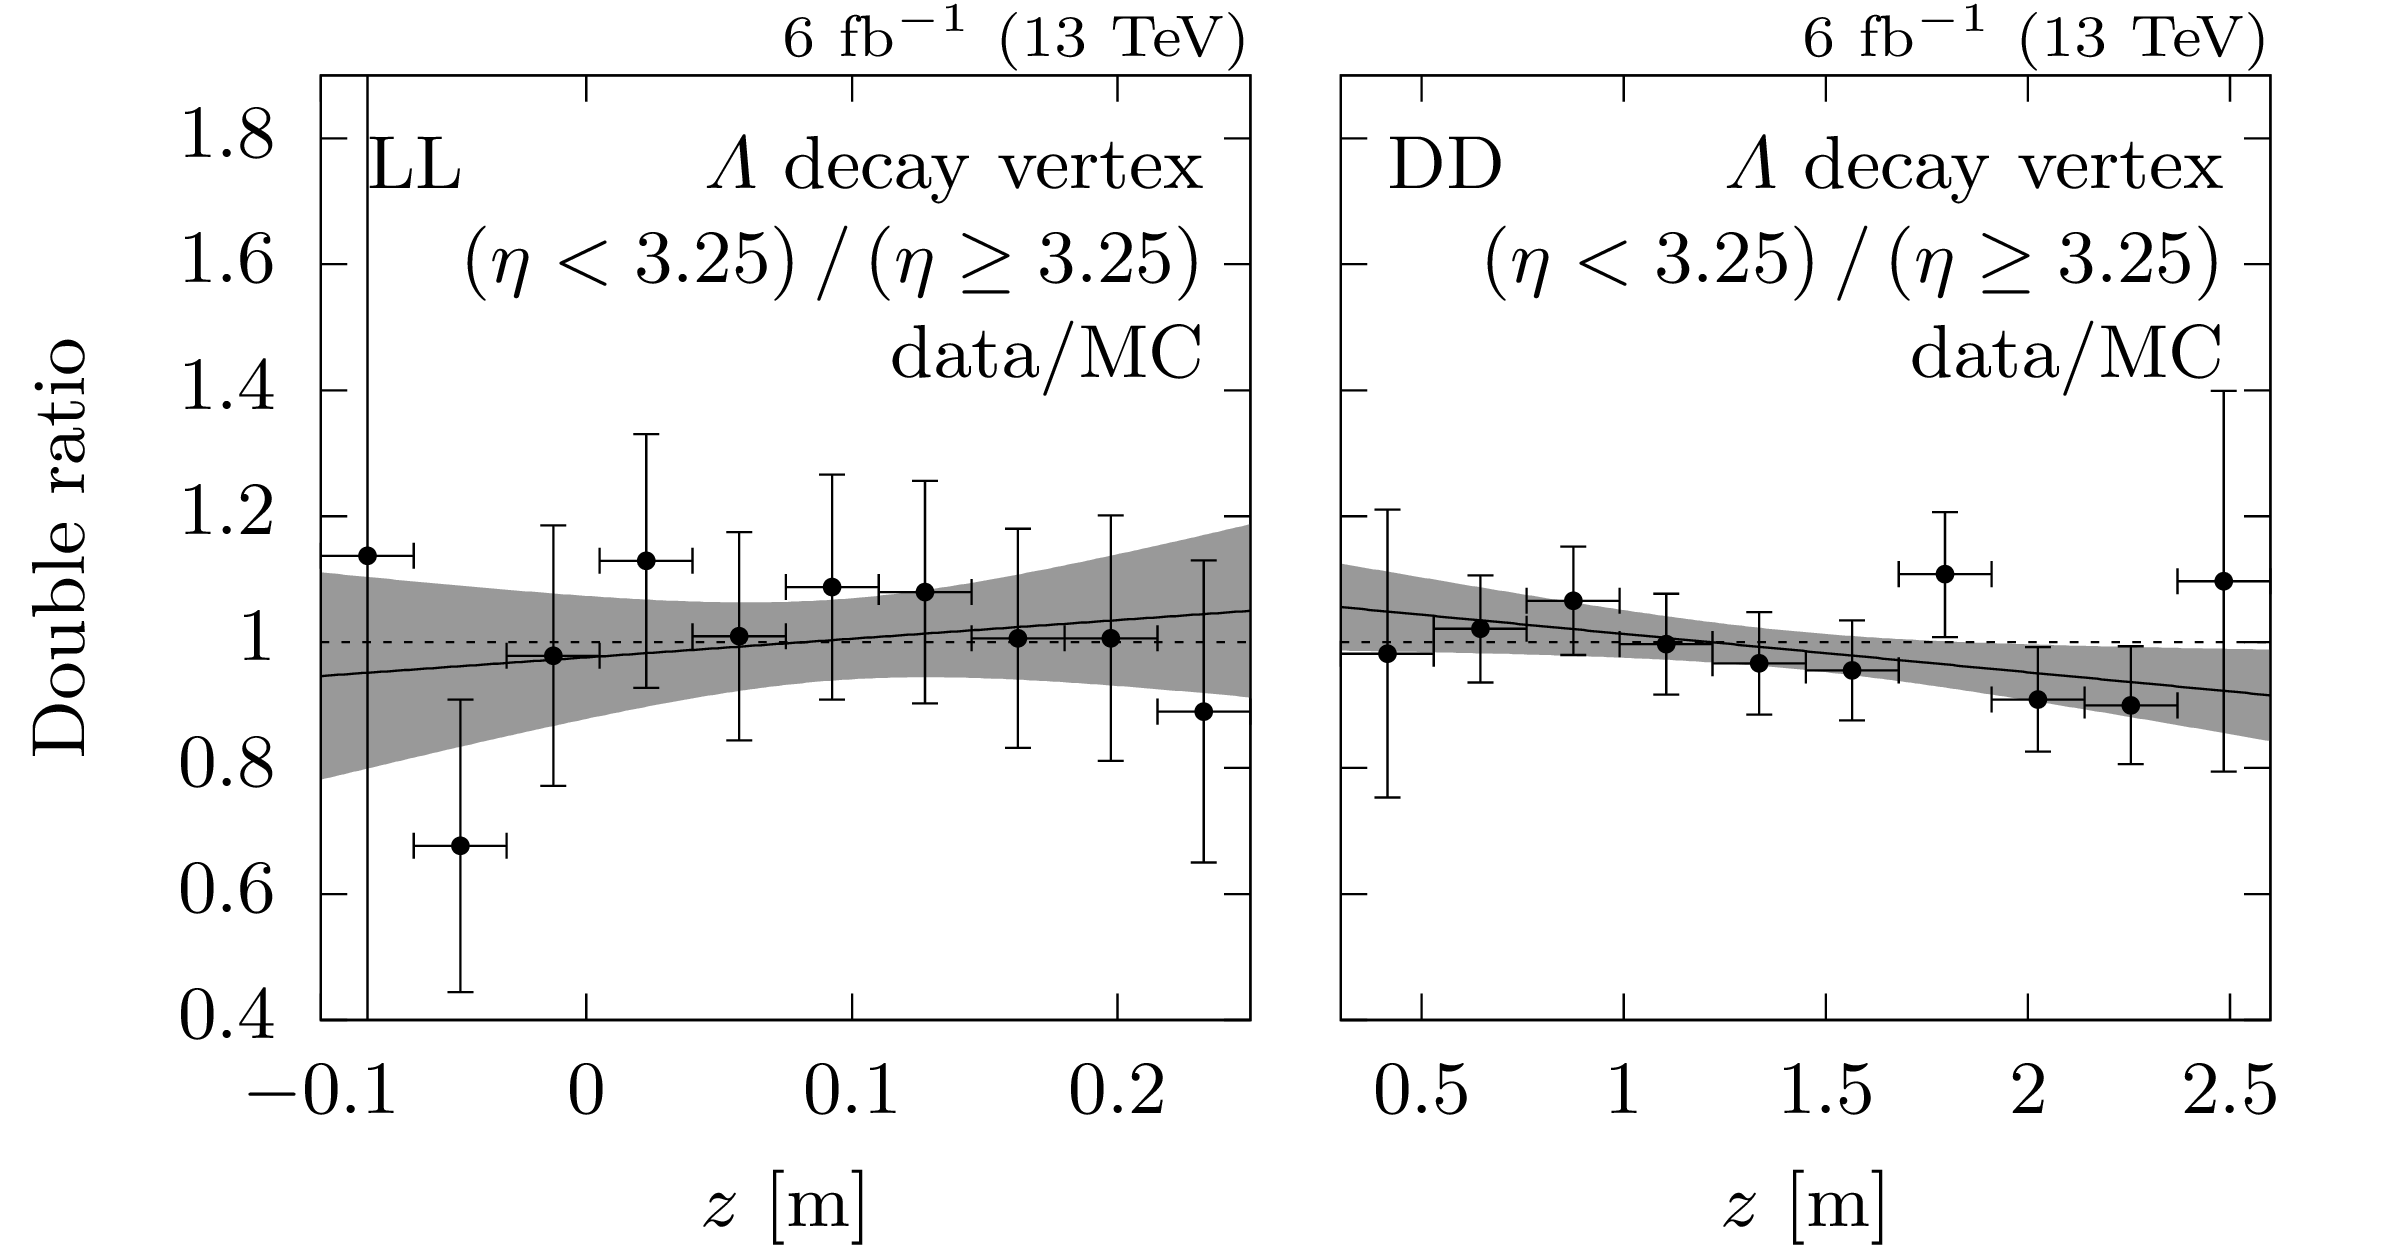
\includegraphics[scale=1.]{Lb2JpsiLz_weighting/hdratio_Lz_endvtx.png}
    \caption{Normalized double ratio of $(\eta < 3.25) / (\eta \ge 3.25)$ and rec.\ data $/$ \gls{mc} sim.\ events as a function of the $z$-position of the \Lz decay vertex for \gls{LL} (left) and \gls{DD} (right) tracks.}
    \label{fig:LbToJpsiLz_hdratio_Lz_endvtx}
\end{figure}

\section{Influence of $\chi^2_\text{DTF}$}
In order to exclude that the difference between \gls{LL} and \gls{DD} tracks is introduced by the $\chi^2_\text{DTF}$ selection criterion, we compare the distribution of the ratio of recorded data and simulated events, parametrized in $\eta(\Lb)$, for $\chi^2_\text{DTF}/\text{\gls{dof}}$ below and above the respective $50\,\%$ quantiles of \gls{LL} and \gls{DD} tracks.
The ratios are shown in Fig.~\ref{fig:LbToJpsiLz/hratio_q50_chi2} and unveil the very same deviation that was observed previously between \gls{LL} and \gls{DD} tracks for small values of $\eta$ in both $50\,\%$ quantiles.
We therefore exclude the hypothesis that $\chi^2_\text{DTF}$ selections introduced the observed deviation.

\begin{figure}[htbp]
    \centering
    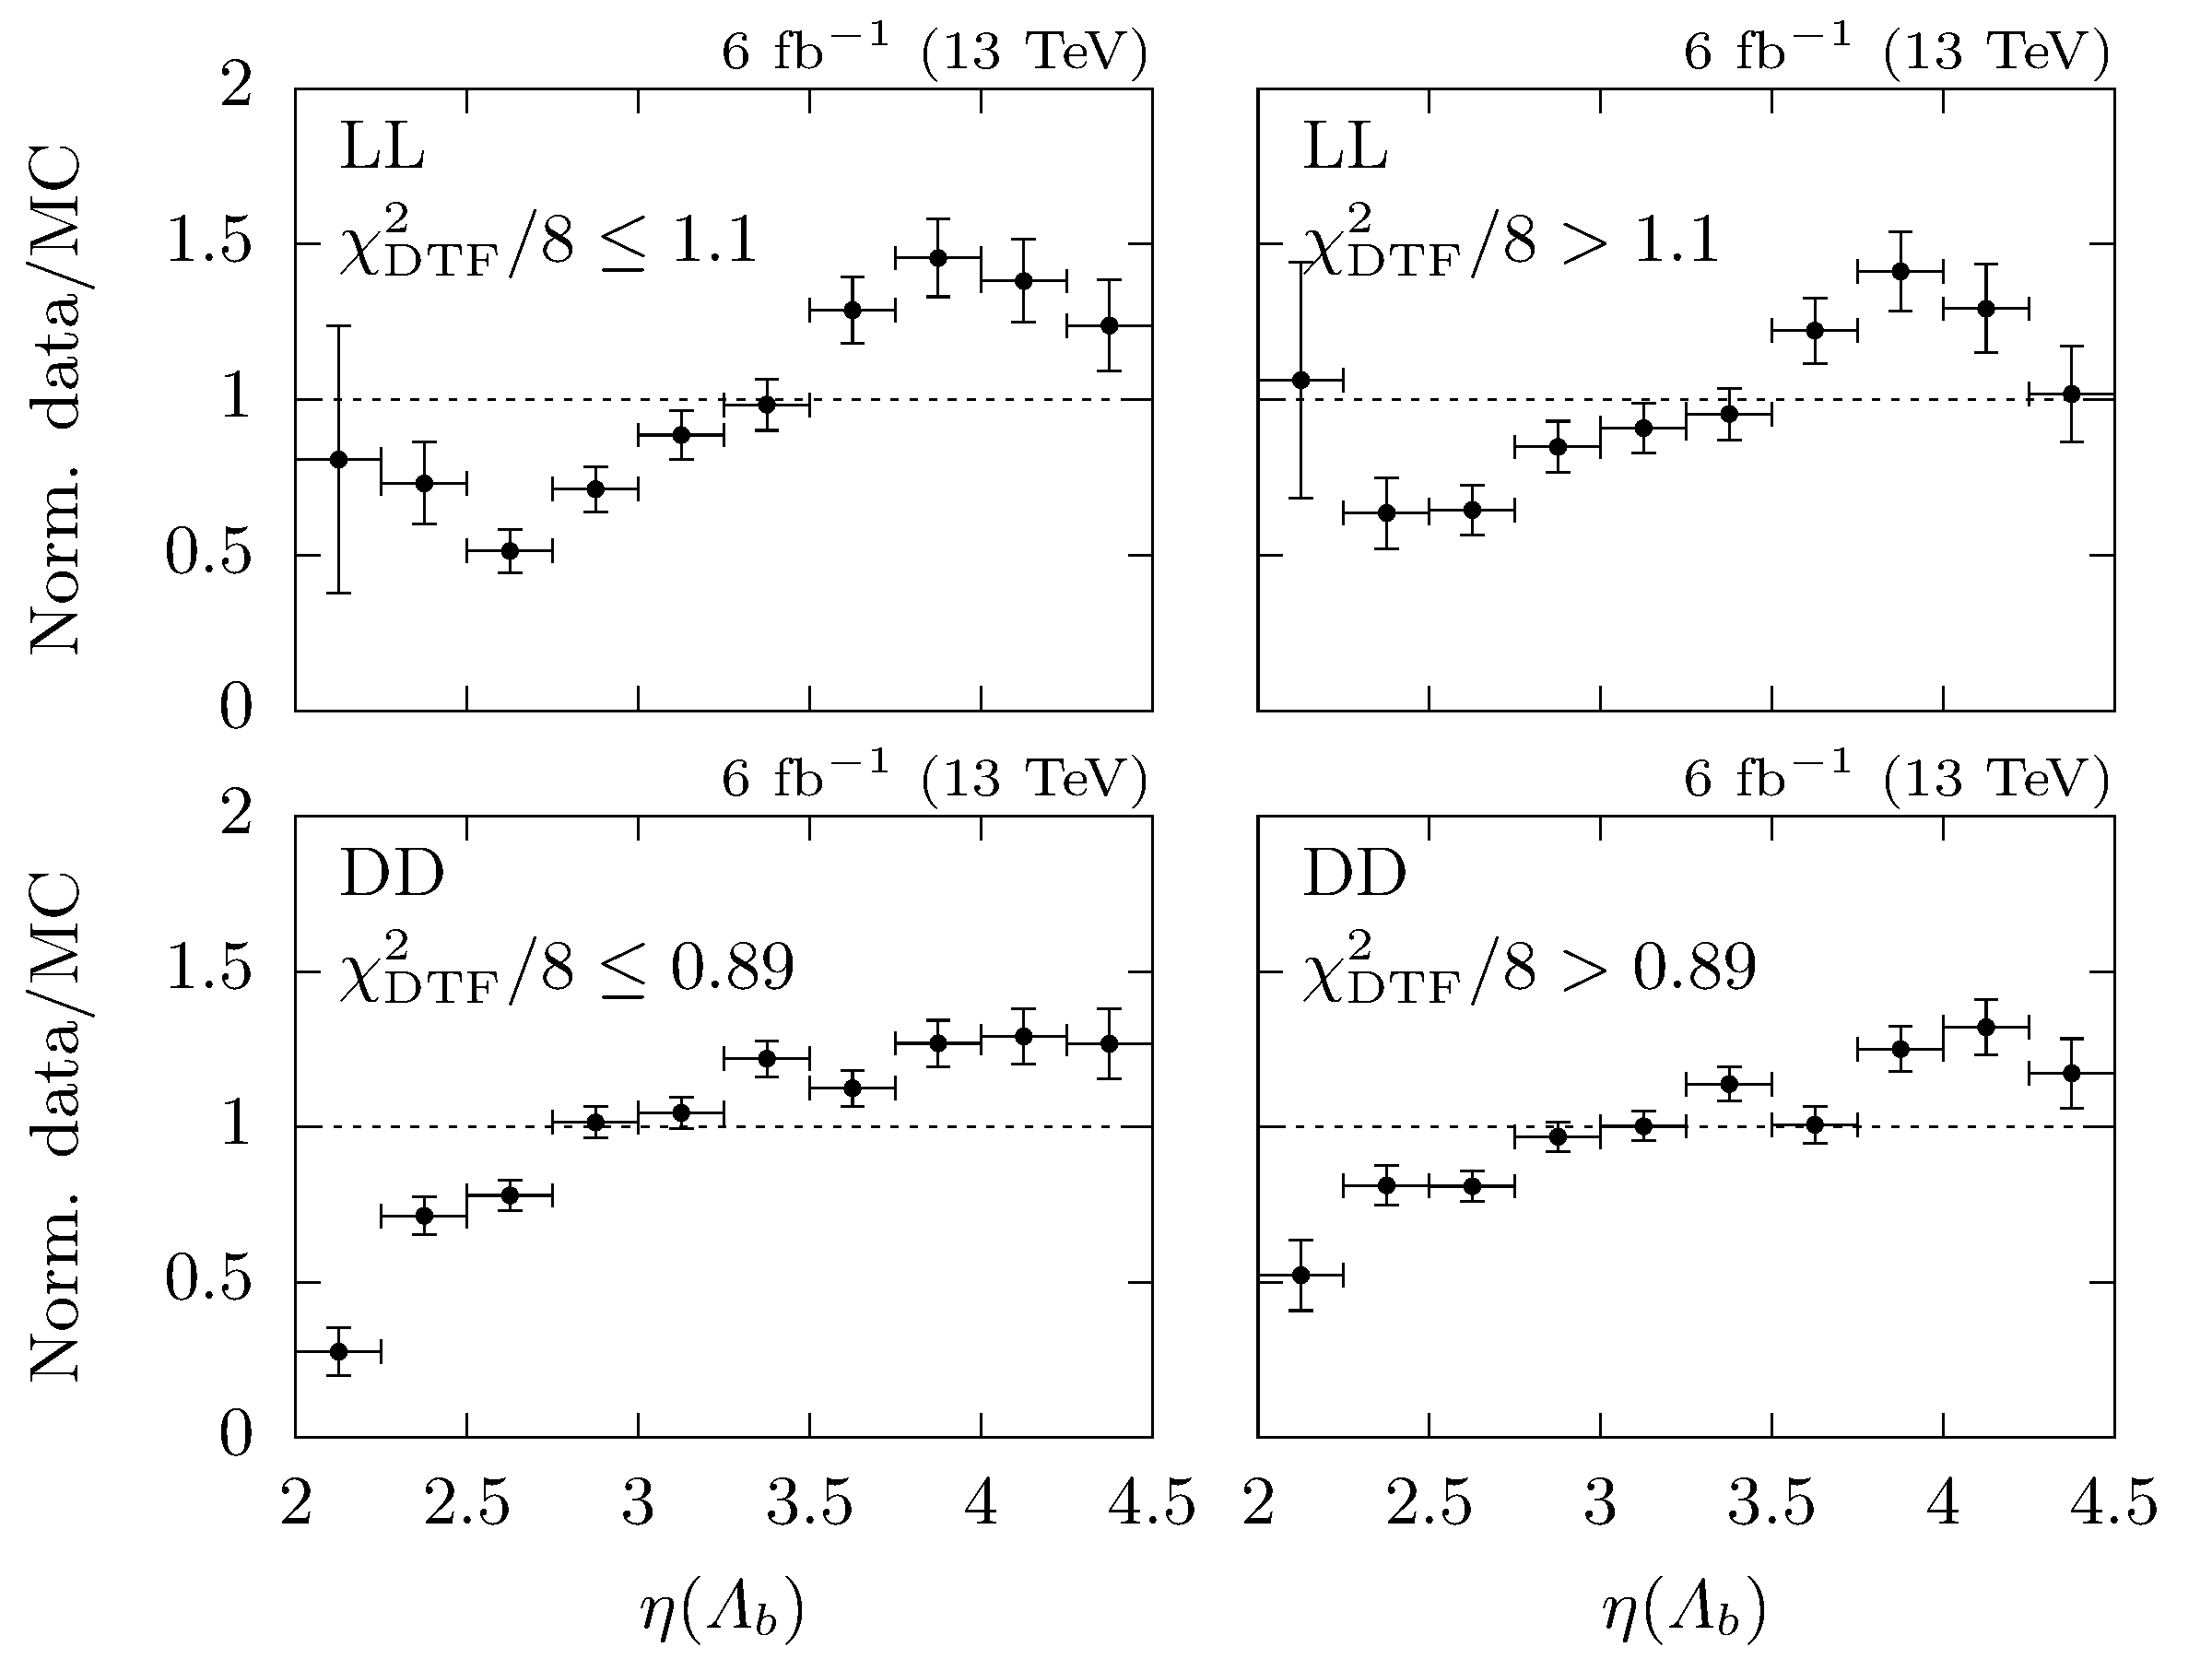
\includegraphics[scale=1.]{Lb2JpsiLz_weighting/hratio_q50_chi2.png}
    \caption{Ratios of recorded data and simulated events, parametrized in $\eta(\Lb)$ for lower and upper $50\,\%$ quantiles of $\chi^2_\text{DTF}/\text{\gls{dof}}$.}
    \label{fig:LbToJpsiLz/hratio_q50_chi2}
\end{figure}

\section{Influence of temporal changes during data taking}
\gls{mc} simulated events are only available for the years 2015 and 2016, whereas we use the full data set of recorded data of \gls{runtwo} in order to increase the significance of the extracted weights.
Since neither the center of mass energy, nor major changes to the apparatus separate the data recorded in the years 2015 and 2016 from those recorded in 2017 and 2018, the same set of weights is expected when using recorded data of the years 2015 and 2016 only, albeit with larger uncertainties.
In Fig.~\ref{fig:LbToJpsiLz_hratio_year} we show $w_2(\eta)$ only using recorded data of the years 2015 and 2016.

\begin{figure}[htbp]
    \centering
    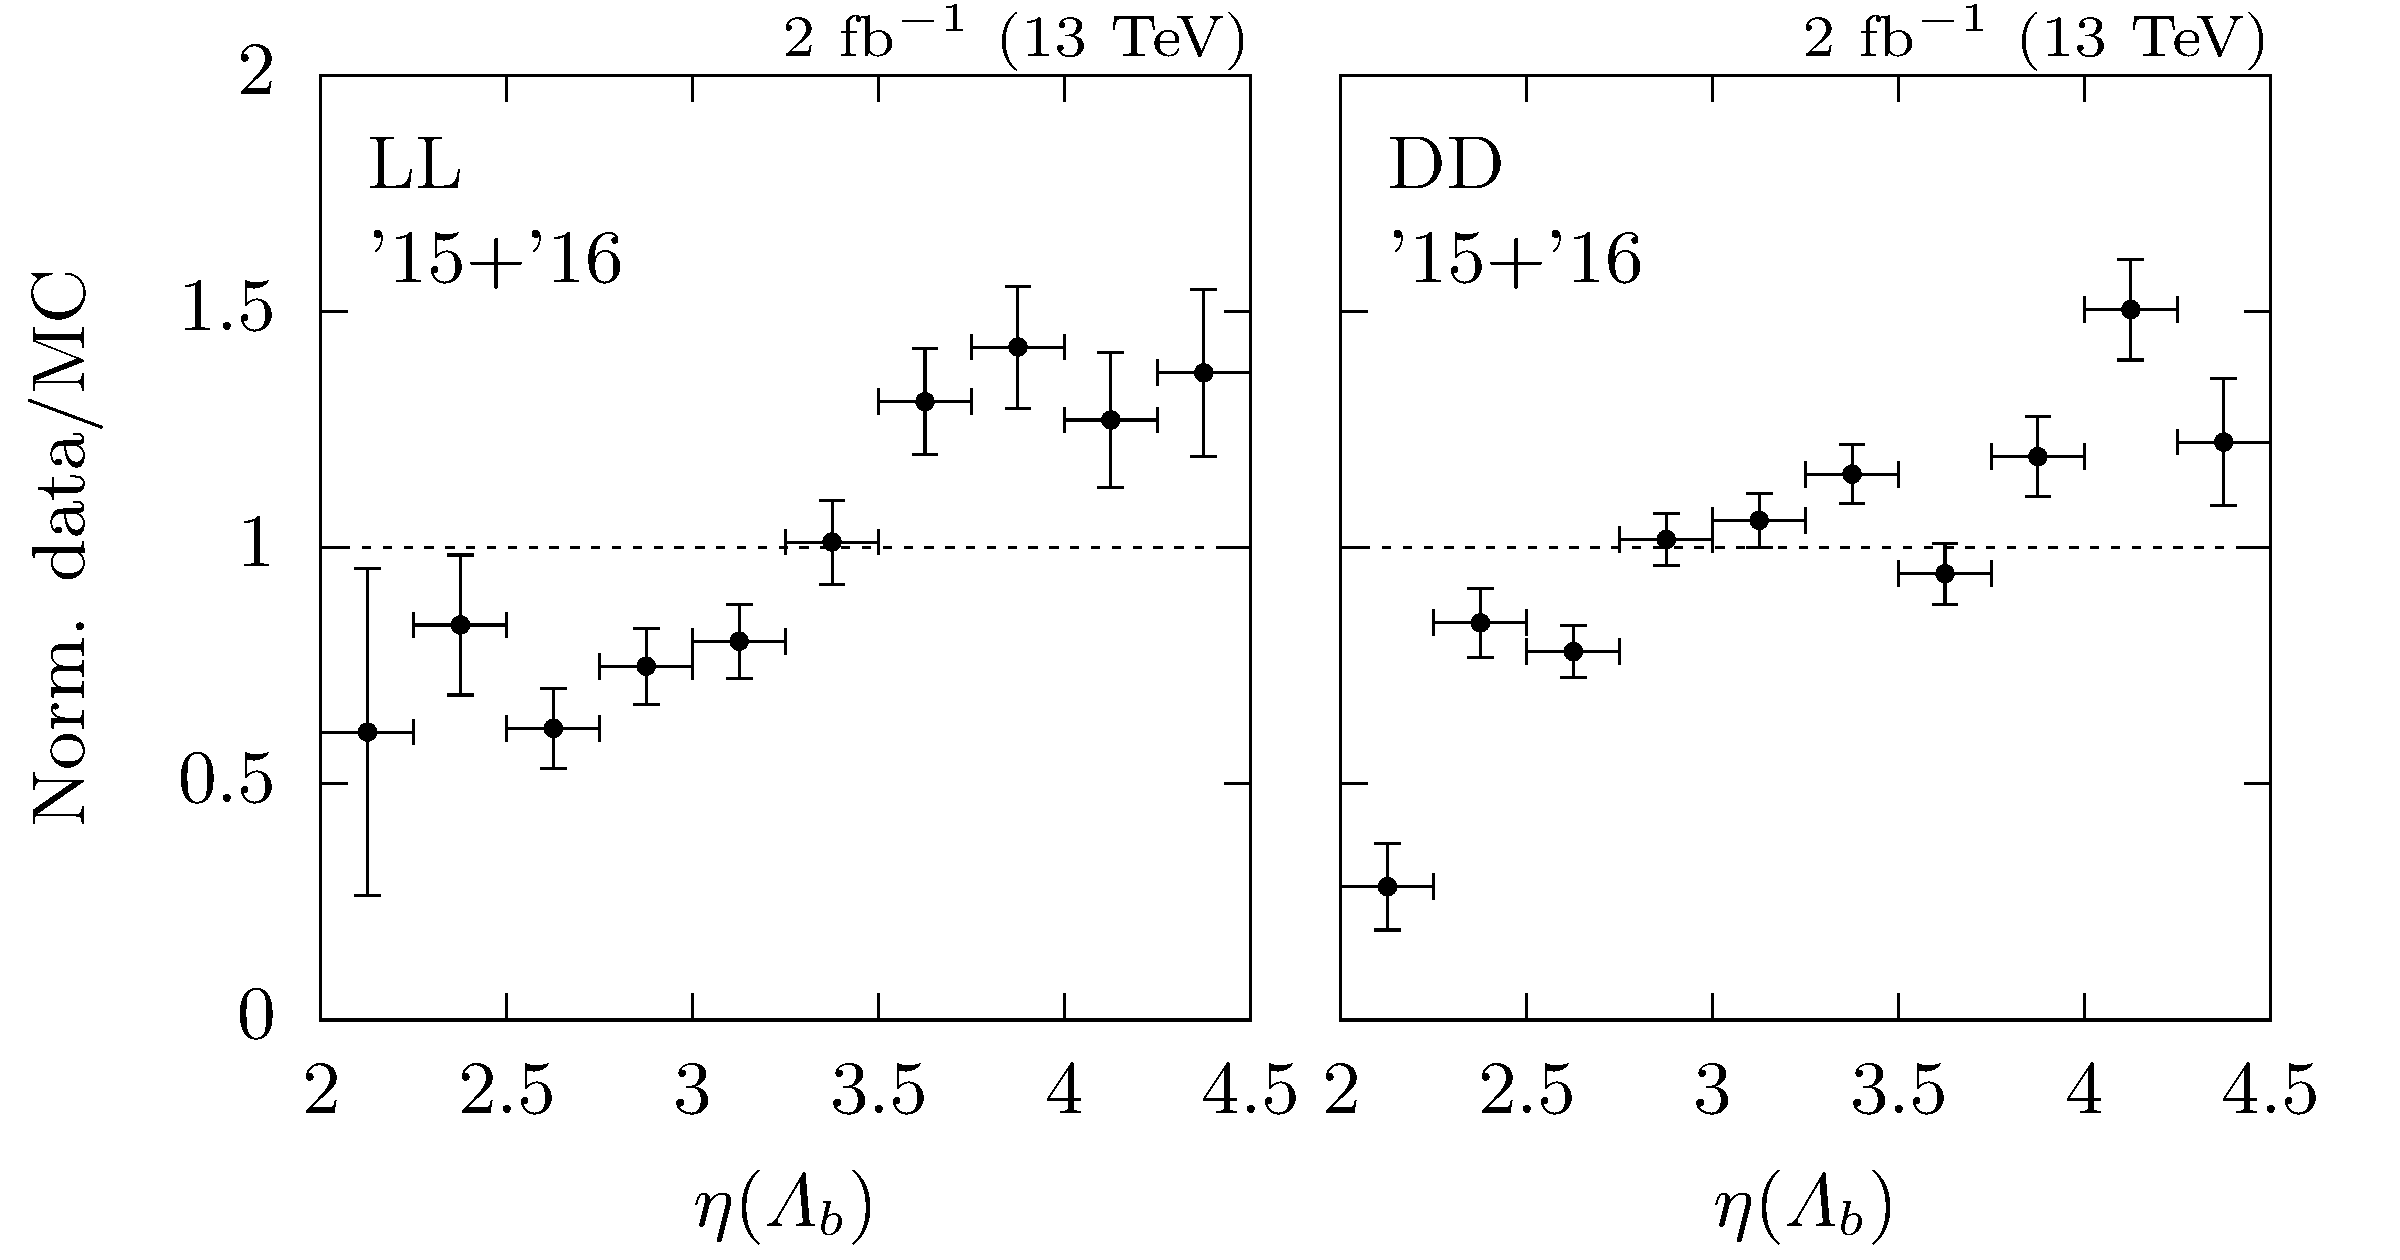
\includegraphics[scale=1.]{Lb2JpsiLz_weighting/hratio_year.png}
    \caption{Weighting factor $w_2(\eta)$ for \gls{LL} (left) and \gls{DD} (right) tracks found by using recorded data of the years 2015 and 2016 instead of full \gls{runtwo} data.}
    \label{fig:LbToJpsiLz_hratio_year}
\end{figure}

Further, we check the impact of magnet polarity and splitting w.r.t.\ the sign of magnet polarity and proton charge ($+1$ for \proton and $-1$ for \antiproton) on the observed accumulation of events for $\eta(\Lb) \gtrapprox 3.25$ and \gls{LL} tracks, and show the corresponding distributions of $w_2(\eta)$ in Fig.~\ref{fig:LbToJpsiLz_hratio_polpid}.
The accumulation in the subsample for a negative product of proton charge and magnet polarity, $Q(p) \times \text{pol.} < 0$, appears pronounced in comparison with $Q(p) \times \text{pol.} > 0$, indicating an misalignment or dead pixels in the left detector hemisphere in a up- to downstream orientation.
(Mag.\ up\ and mag.\ down\ are associated with $+1$ and $-1$, respectively.)
However, these effects are insignificant and it is unclear why they seem to be absent in \decay{\Lb}{\Dz\proton\pim} but are not correlated with the $z$-position of the $\Lz$ decay vertex.

\begin{figure}[htbp]
    \centering
    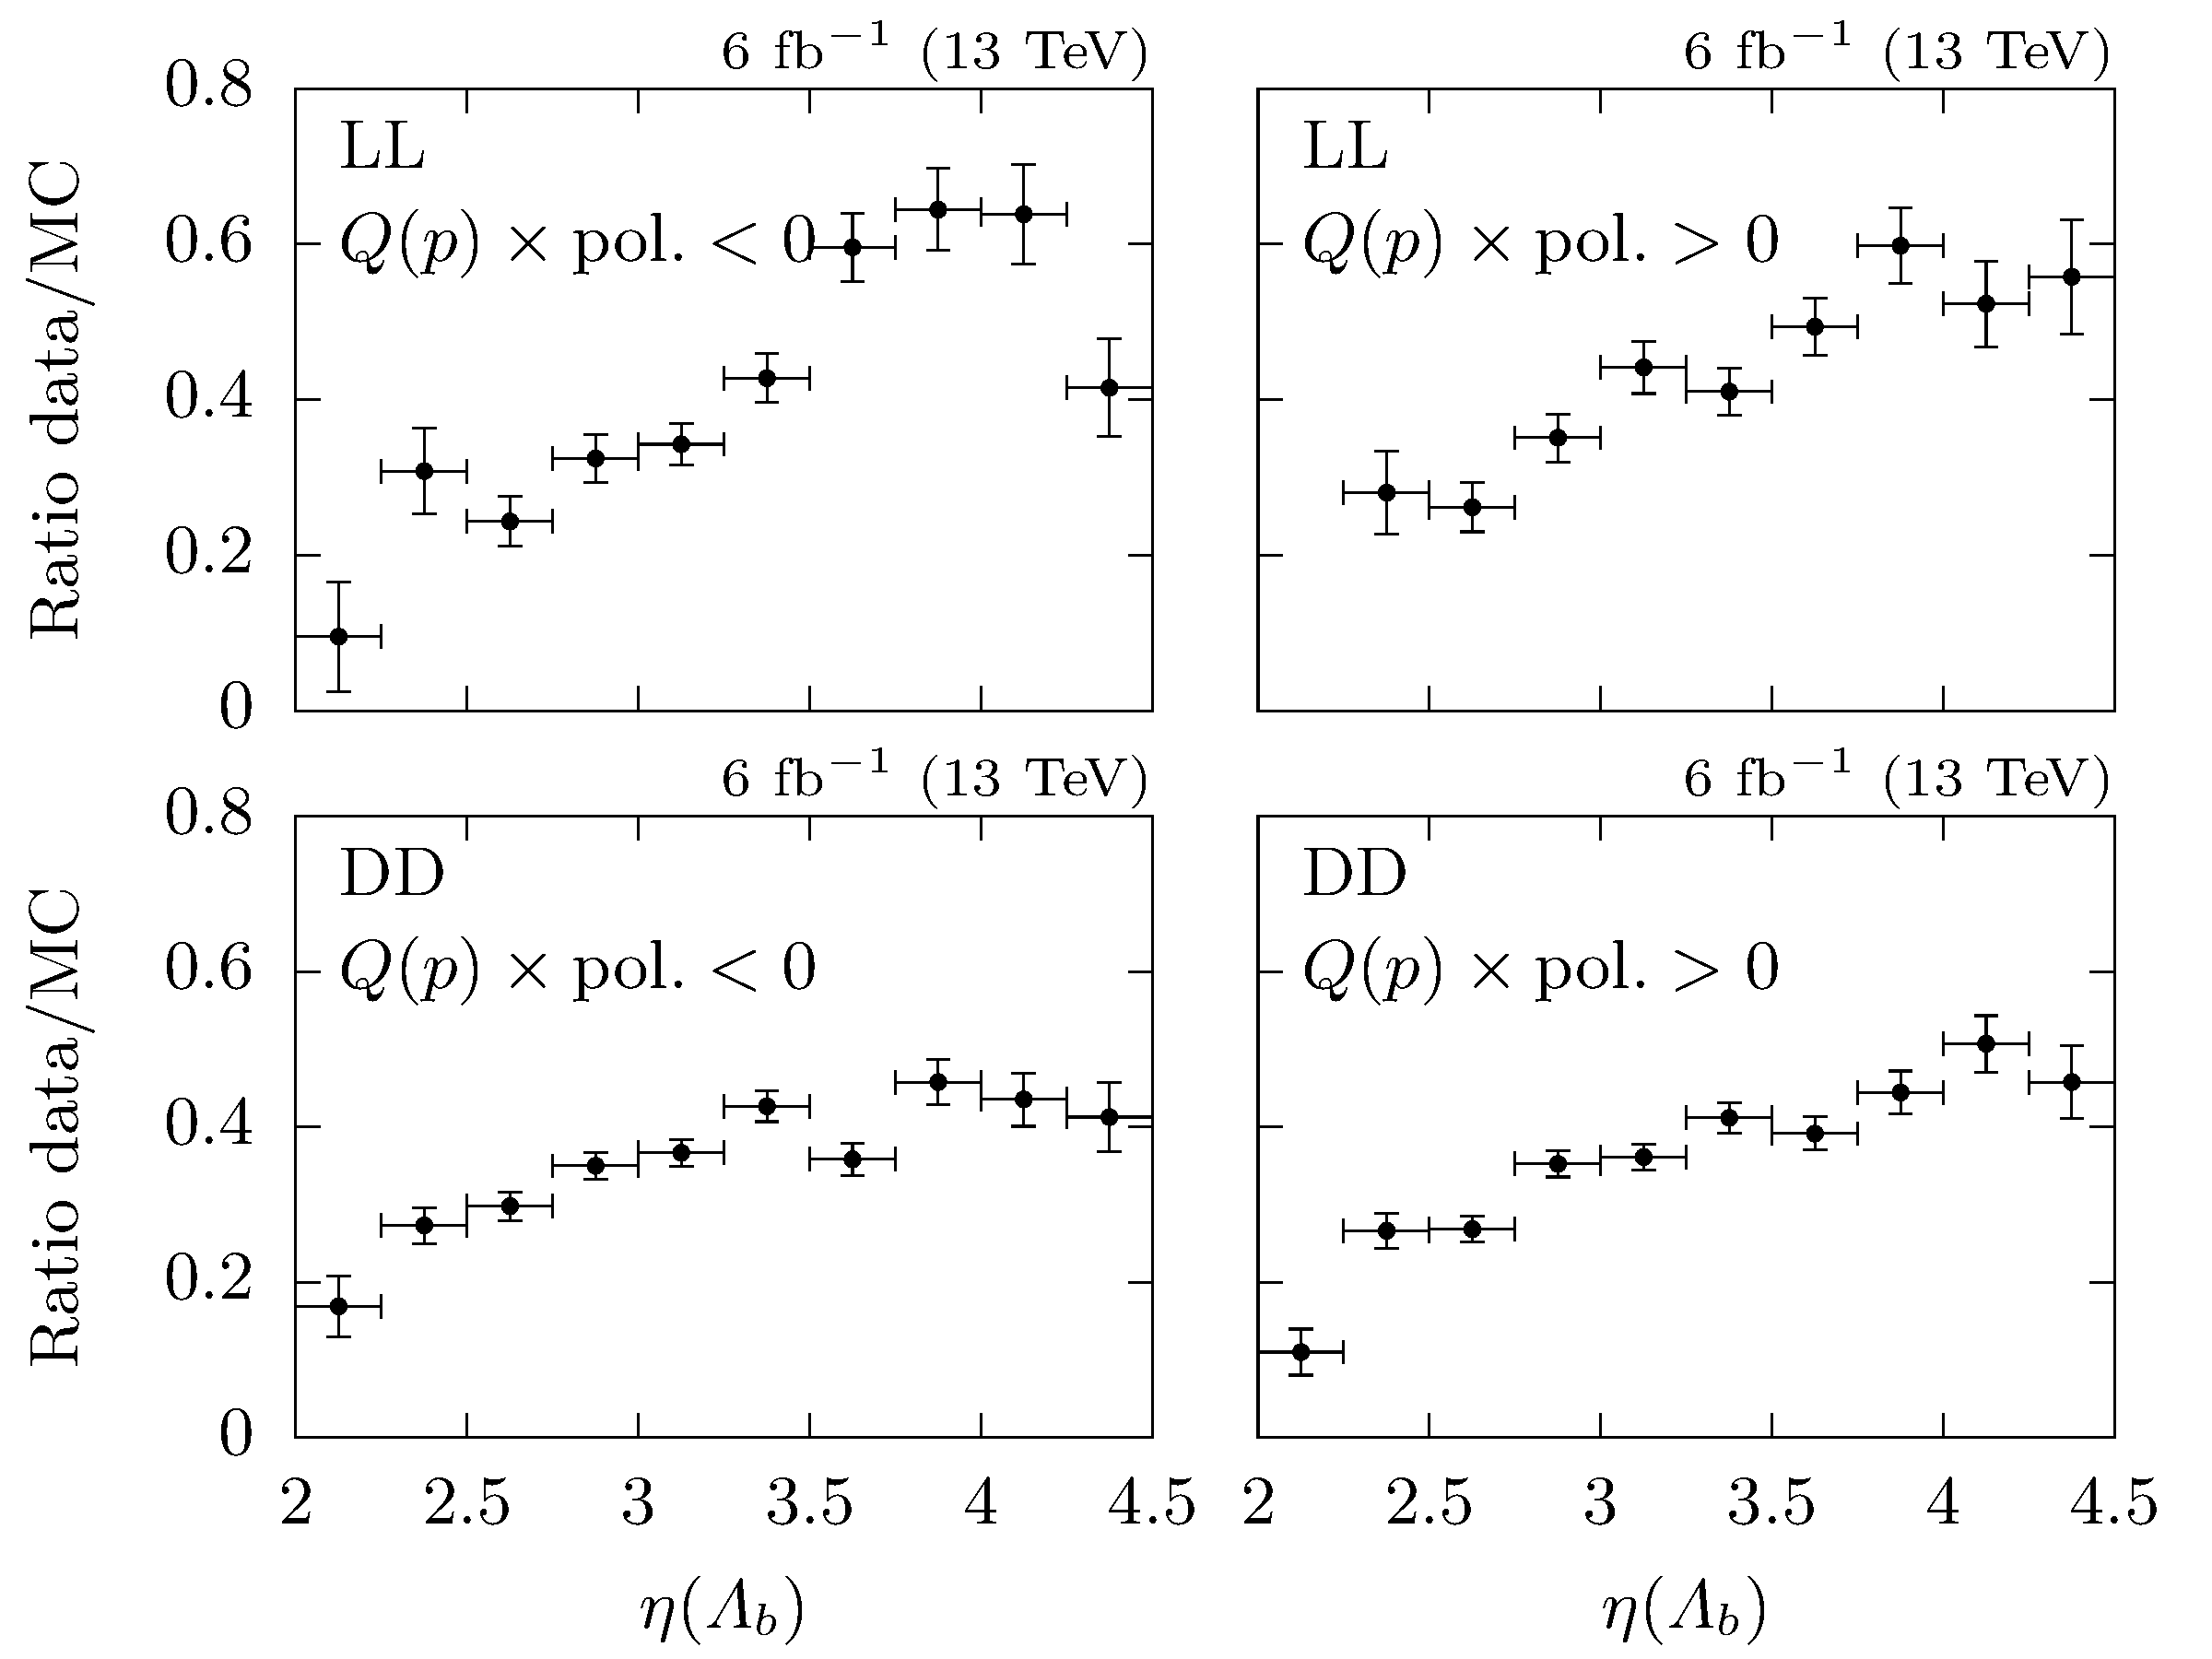
\includegraphics[scale=1.]{Lb2JpsiLz_weighting/hratio_polpid.png}
    \caption{Samples split w.r.t.\ the sign of the product of proton charge and magnet polarity.}
    \label{fig:LbToJpsiLz_hratio_polpid}
\end{figure}

\section{Summary}
The reason for the deviation stays unclear.
For the decay \decay{\Lb}{\jpsi\Lz} (\gls{lzero} \gls{tis} triggered), this effect could be a statistical fluctuation, due to misalignment effects that are not reproduced well in the simulated events, or other reasons.
The deviation w.r.t.\ \decay{\Lb}{\Dz\proton\pim} decays (\gls{lzero} \gls{tos} triggered) is significant but the reason also stays unclear.
Further it is unclear, whether \gls{tos} triggered \decay{\Lb}{\Dz\Lz} will be distributed similar to \decay{\Lb}{\jpsi\Lz} and \decay{\Lb}{\Dz\proton\pim} or deviate from both.
(It is worthwhile to mention that for perfect simulations there should not be any deviation in any of these samples.)
